% Page couverture du document de reference

\pagestyle{empty}

\textblockorigin{0mm}{0mm}
\setlength{\parindent}{0mm}

\begin{textblock*}{\paperwidth}(0mm,0mm)
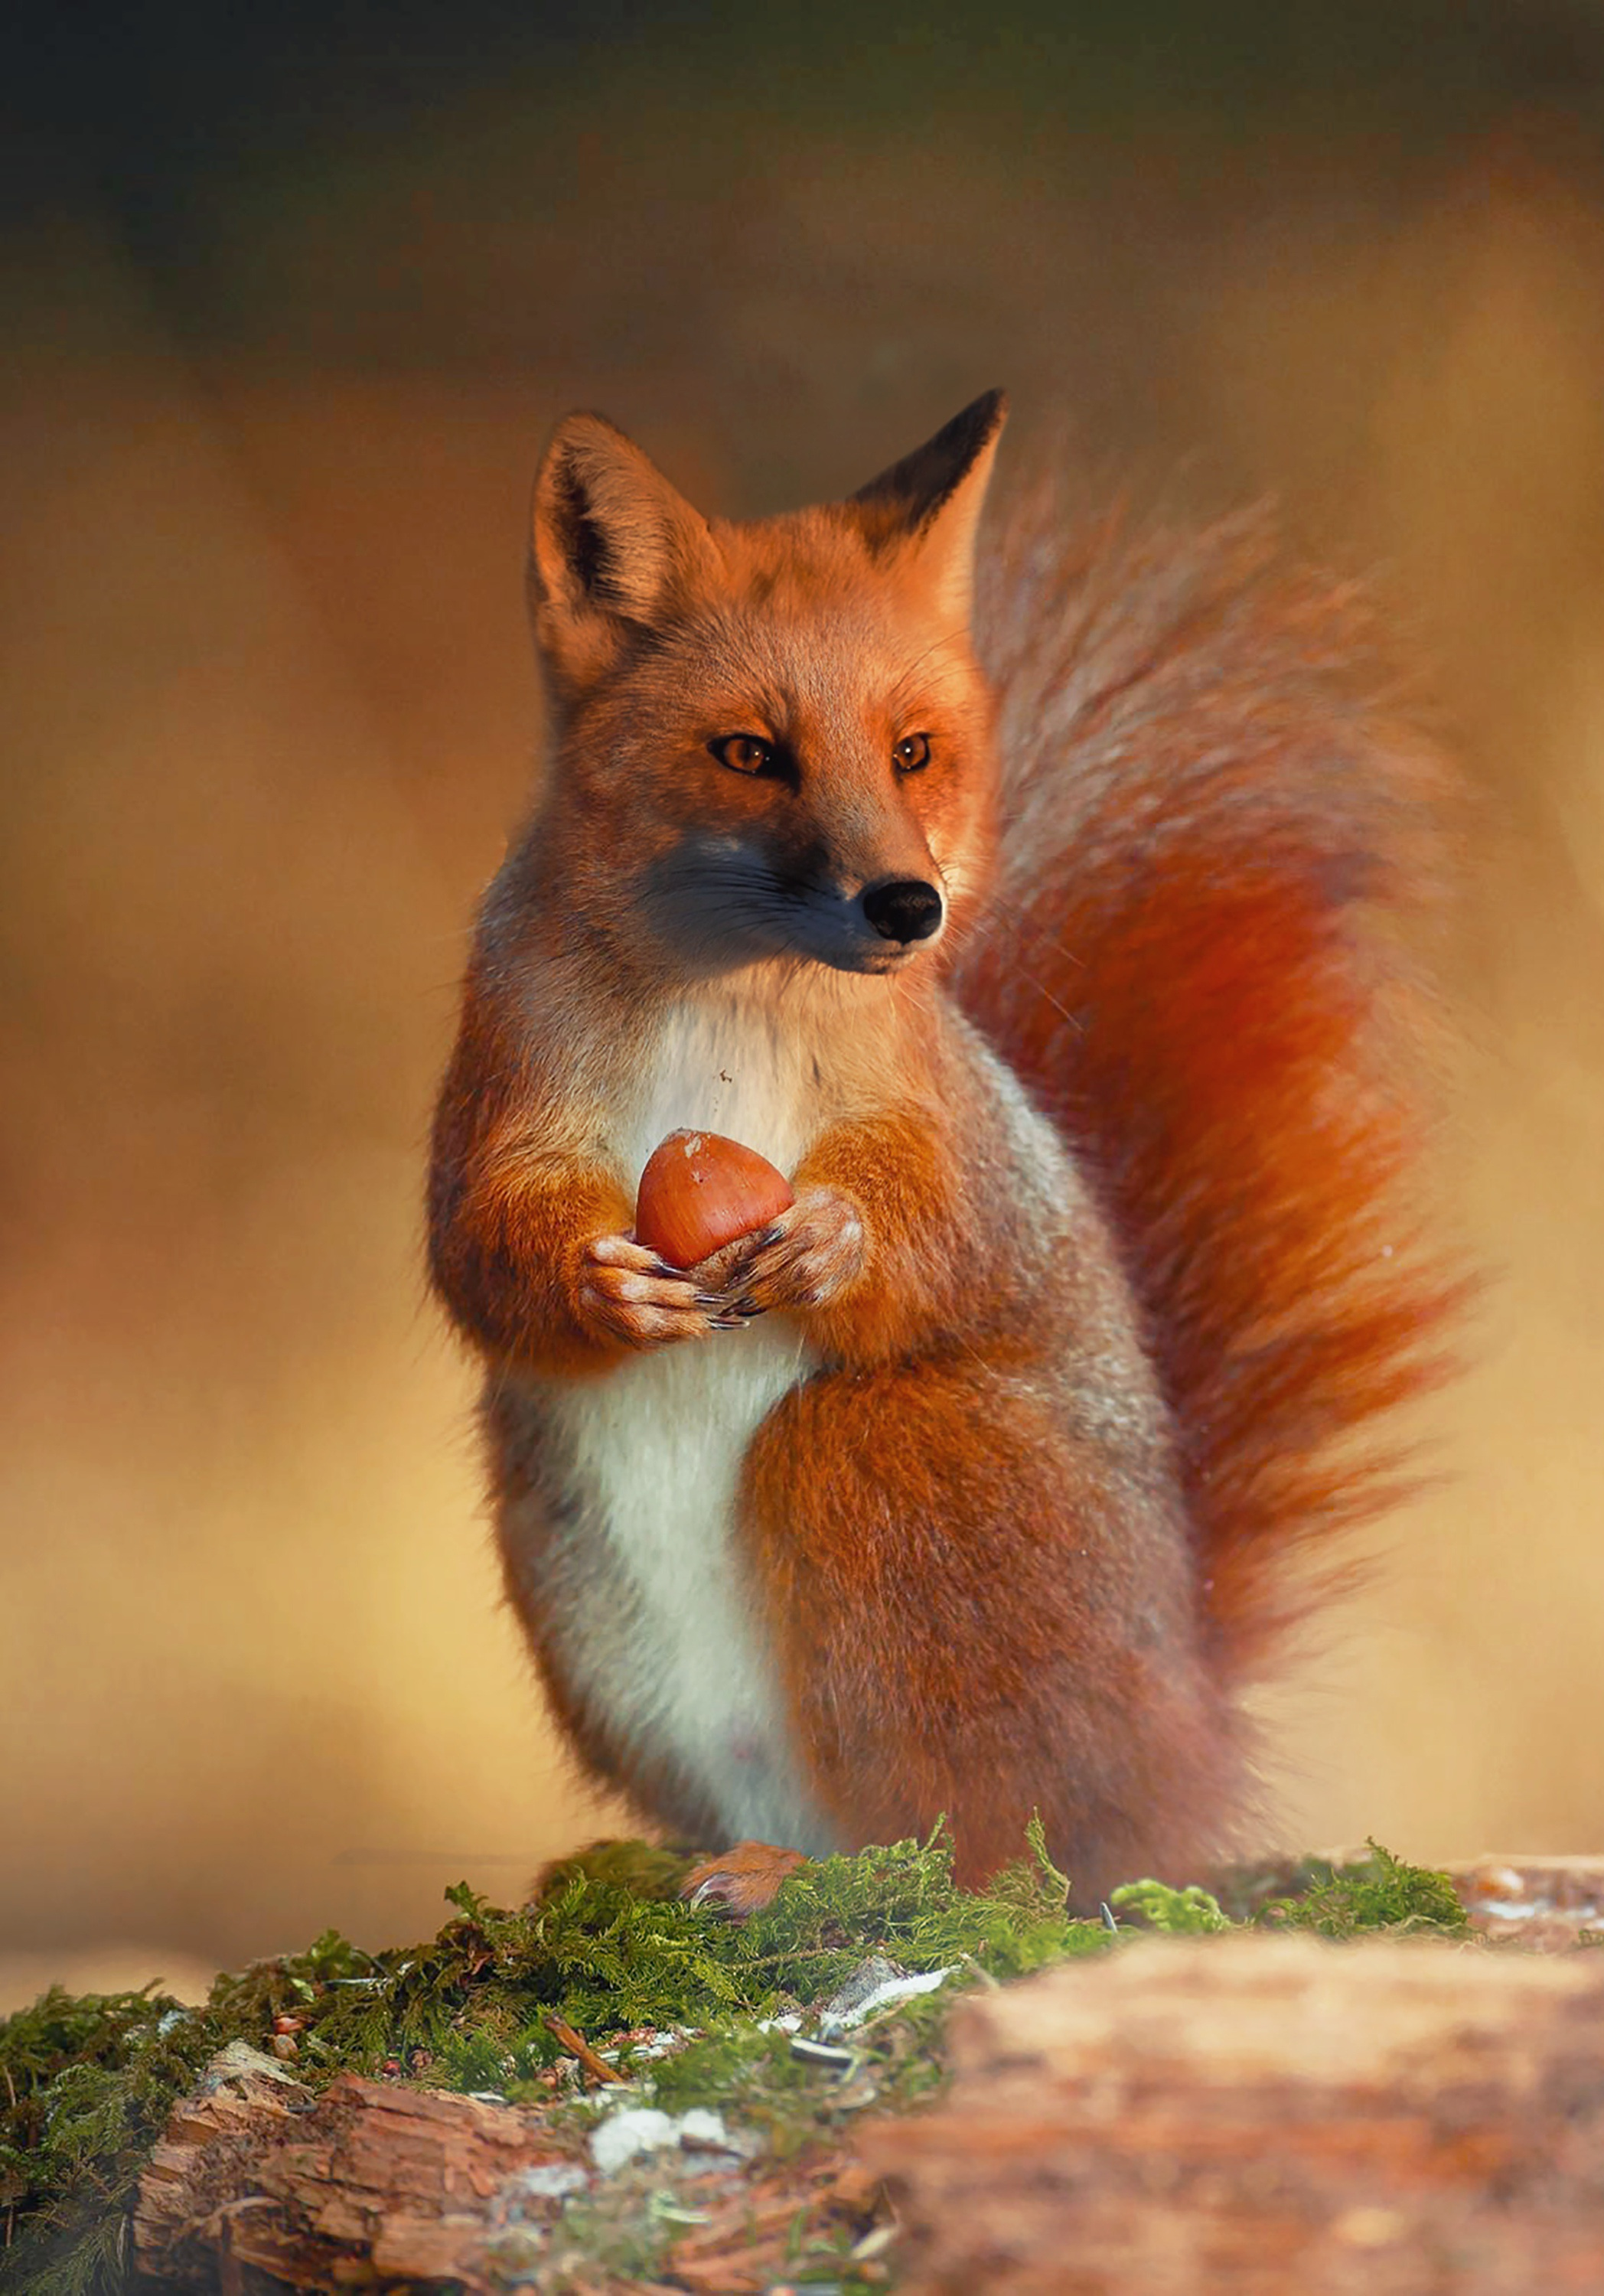
\includegraphics[height=11in, width=\paperwidth]{src/GuideEnActuariat/couverture.jpg} \\
\end{textblock*}

\begin{textblock*}{500mm}(30mm,10mm)
% \sffamily
% \bfseries\fontsize{65}{42}\selectfont
{ \color{white} 
\TITLE
}
\end{textblock*}

\null\newpage

% ------------------------------------------
% Deuxième page : présentation des auteurs et liens vers le dépôt Github du guide
% ------------------------------------------
\begin{textblock*}{\paperwidth}(20mm,40mm)
\raggedright
\TITLE
\end{textblock*}

\begin{textblock*}{\paperwidth}(20mm,100mm)
\raggedright
\AUTHORS
\end{textblock*}


\begin{textblock*}{\paperwidth}(20mm,210mm)
\raggedright
\href{https://github.com/NicholasLangevin/Guide_de_survie_en_actuariat}{Dépôt officiel de ce document} \\
Dernière mise à jour : \today
\end{textblock*}

\null\newpage
